
\chapter{Estado del arte}\label{cap:edoarte}

%Que se está utilizando en la literatura o en el mercado para implementar tableros de datos
%Hablar de software Open Source y de paga mencionando ventajas y desventajas de cada uno. También explicar porque cada software no es viable para la solución.

El presente capítulo tiene como objetivo realizar una revisión crítica y sistemática de la literatura y el mercado actual en torno a la implementación de tableros de datos. Se analizará el uso de software \textit{Open Source} y de pago, considerando sus ventajas y desventajas, con el fin de determinar la mejor opción para la implementación de un tablero de datos en el contexto del presente trabajo.\\

Se presentará una revisión de las principales herramientas \textit{Open Source} disponibles para la creación de tableros de datos, como Tableau Public, Google Data Studio y Grafana. Se describirán sus características, ventajas y desventajas. De manera similar, se analizarán las principales herramientas de pago disponibles para la creación de tableros de datos, como Microsoft Power BI, Tableau y Domo.



\section{Software para tableros de datos}\label{sec:seccion3.1}
Un software para la implementación de tableros de datos, es una plataforma centralizada que permite a las empresas e instituciones visualizar y analizar información compleja de forma simplificada e intuitiva. Ayudan a presentar los datos en un formato visualmente atractivo e interactivo, lo que permite a los usuarios supervisar los indicadores clave de rendimiento \textit{(KPI)} y obtener información procesable para tomar decisiones informadas \cite{wexler2017big}.

En esencia, este tipo de software actúa como puente entre los datos brutos y la información significativa. Transforma conjuntos de datos complejos en representaciones visuales comprensibles. Esto facilita a los usuarios la comprensión e interpretación de la información. Los tableros suelen consistir en diagramas, gráficos, tablas y otros elementos visuales que condensan grandes volúmenes de datos en visualizaciones concisas y significativas \cite{kirk2016data} \cite{kerzner2015dashboard}. \\

Las principales características que se buscan en un software para el desarrollo de tableros son las siguientes \cite{wexler2017big}:

\begin{enumerate}
    \item \textbf{Plantillas de tableros predeterminadas y opciones de estilos}\\
    Esta característica permite a los usuarios elegir entre plantillas prediseñadas y personalizar el estilo del tablero para adaptarlo a sus necesidades.
    
    \item \textbf{Seguridad de los datos}\\
    Este es un aspecto importante a tener en cuenta antes de elegir la herramienta adecuada. Garantizar que los datos confidenciales de la institución están protegidos en todo momento es de gran importancia, no sólo por razones de seguridad, sino también porque las normativas de seguridad son cada vez más estrictas.
    
    \item \textbf{Procesamiento de datos en tiempo real}\\
    Un tablero tiene como uno de sus propósito proporcionar las tendencias generales al tiempo que permite a los usuarios la capacidad de desglosar y acceder a múltiples capas de datos.
    
    \item \textbf{Personalización e integración}\\
    Un tablero que puede ser personalizable permite a los usuarios elegir qué puntos de datos y visualizaciones pueden ver, mientras que la integración con otras herramientas permite mejorar los análisis e informes.

    
    \item \textbf{Gráficos}\\
    Un buen software para desarrollo de datos debe de proporcionar gráficas personalizables que ayudan a transmitir las métricas esenciales de forma rápida y atractiva.

    \item \textbf{Opciones para compartir}\\
    Un buen software suele proveer diversas opciones para compartir tableros entre diferentes personas. Esto se puede hacer mediante el inicio de sesión desde otro dispositivo, el envío de tableros e informes por correo electrónico, o el uso de un visor externo.

    \item \textbf{Capacidad de exportación e impresión}\\
    Esta característica permite poder exportar los tableros en archivos con formato PDF o PNG sin que el tablero pierda su estructura y diseño al momento de la conversión.
    
    
\end{enumerate}





\section{Software Open Source}
La implementación de tableros de datos utilizando tecnología de código abierto tiene muchas ventajas que los convierten en una opción sustentable para muchas organizaciones. A continuación se analizarán algunas de los principales software \textit{open source} que se utilizan para la creación tableros de datos creados con tecnología de código abierto, junto con ejemplos de algunos de los principales casos de uso para los que se ha utilizado dicha tecnología.

\subsection{Tablueau Public}
Tableau Public es una plataforma gratuita para explorar, crear y compartir públicamente tableros para la visualización de datos en línea. Cualquier persona puede crear tableros utilizando la aplicación web.\\
Se pueden procesar datos en diversos formatos, como Excel, CSV y Google Sheets, para crear visualizaciones atractivas e interactivas con una interfaz fácil de usar la cual no requiere de la producción de código \cite{tableau_public_about}.\\

La razón principal por la cual esta opción no es viable para la implementación de este proyecto, se debe a que los datos pueden ser observados por cualquier persona, lo cual no de debería ser posible ya que se manipulan datos privados y delicados que no son de uso público.

\subsection{Grafana}
Grafana es una aplicación web de análisis y visualización interactiva multiplataforma. Proporciona tablas, gráficas y alertas para la web cuando se conecta a fuentes de datos compatibles. Es principalmente una herramienta de visualización que proporciona gráficos interactivos para administradores y tableros de datos alimentados por flujos de entrada de datos.\\
Grafana cuenta con un modelo de fuente de datos conectable que puede conectarse con una amplia gama de fuentes de datos, incluidos datos de series temporales, pero también bases de datos relacionales como lo MySQL y PostgreSQL \cite{mccollam2022getting}.\\

La razón por la cual se descartó su uso para este proyecto se debe la curva de aprendizaje es grande. La configuración de los plugins puede requerir un esfuerzo considerable. Las opciones de configuración a través de la interfaz gráfica de usuario son limitadas y a menudo es necesario el mantenimiento y la edición manual de los archivos de configuración.


\subsection{Google Data Studio}
Google Data Studio es una herramienta de \textit{Business Intelligence (BI)}, que procesa datos brutos en información estratégica para las empresas e instituciones. A través de la visualización de datos, Google Data Studio reúne métricas e indicadores que apoyan la toma de decisiones y estrategias. Está diseñada para ayudar a los profesionales del marketing, a los propietarios de empresas y a los analistas de datos a visualizar los datos para obtener información y tomar decisiones fundamentadas. Google Data Studio es compatible con más de 150 fuentes de datos, como Google Analytics, Google Ads, Google Search Console, BigQuery, YouTube Analytics y muchas otras \cite{kemp2021google}.\\
Además, esta plataforma permite hacer operaciones sobre los datos al momento de exportarlos. Por ejemplo, si tenemos una columna dónde los datos son fechas en formato \texttt{Unix Timestamp} o en días (DD/MM/YYYY) y el objetivo es mostrar una serie de tiempo, pero agrupada en meses o años, Google Data Studio provee opciones para hacer este tipo de operaciones y más, como la posibilidad de modificar interactivamente los tableros mediante filtros.\\

La razón por la cual no se decidió trabar con este producto de Google se debe a qué es relativamente nuevo y no cuenta con todo el tipo de gráficas que se necesitan para el proyecto y la personalización de estas es limitado.
%-------------------------------------------------------------------


\section{Software de paga}
Habiendo hablado de opciones \textit{Open source} las cuales proveen herramientas provechosas para la implementación y creación de tableros de datos, estas tecnologías son una gran opción si el proyecto en el que se está trabajando no es de una escala considerablemente grande, los datos que se manipulan no son privados o los encargados de la implementación no cuentan con una amplia experiencia en cuestión de programación o con el uso de \texttt{SQL}.\\
Ya que como se pudo observar, todas las opciones mencionadas tienen algún tipo de restricción en cuanto a lo que concierne al proyecto en el que se trabajó. Los datos desplegados en el tablero de datos no son de uso público y las herramientas \textit{Open source} no permiten una personalización extensa.\\

En esta sección se explorarán herramientas por las cuales hay que realizar algún tipo de pago para usarlas, las cuales pueden llegar a ofrecer servicios más extensos y personalizables que los anteriormente vistos.


\subsection{Microsoft Power BI}
Power BI es un conjunto de servicios de software, aplicaciones y conectores que trabajan juntos para convertir diferentes fuentes de datos no relacionadas en perspectivas coherentes, visualmente inmersivas e interactivas. Los datos pueden estar contenidos en una hoja de cálculo de Excel o una colección de almacenes de datos híbridos basados en la nube y locales. Power BI  permite conectarse fácilmente a sus fuentes de datos, visualizar y descubrir lo que es importante, y compartirlo con quien se desee \cite{microsoft_power_bi_overview} \cite{clark2017beginning}.\\

En la Figura \ref{fig:powerBI_ej} se puede observar un tablero de datos con diferentes métricas y datos sobre ventas y marketing, implementado en \texttt{Power BI}.

%\begin{center}
    \begin{figure}[H]
        \centering
        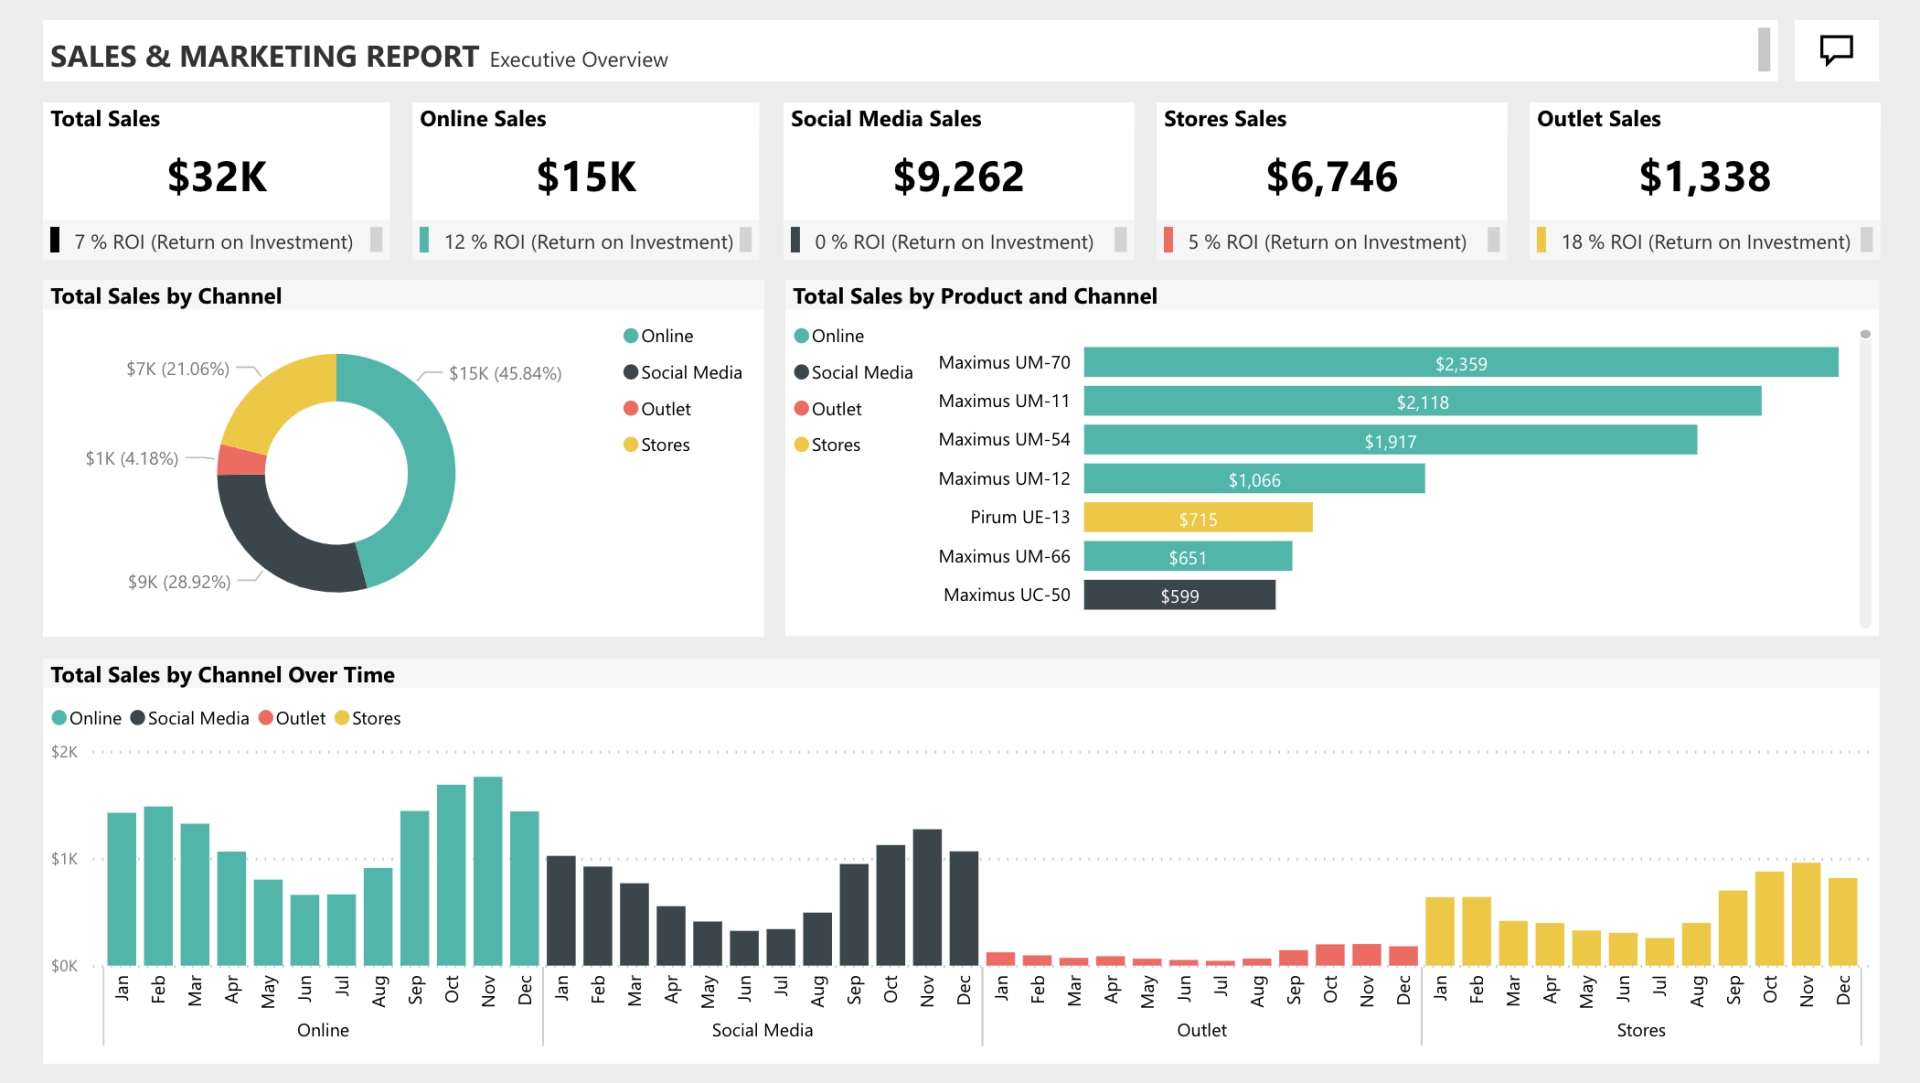
\includegraphics[width=0.8\textwidth]{images/power_bi_ejemplo.png}
        \caption{Ejemplo de un tablero de datos implementando en \texttt{Power BI}.}\label{fig:powerBI_ej}
    \end{figure}
%\end{center}

Una de las características más notorias de este servicio es que puede usar tanto en su página web, en su aplicación local para computadoras y su aplicación para dispositivos móviles Android y iOS. Además de que se puede usar en conjunto con los diferentes productos que Microsoft ofrece.\\
Un diferenciador que resalta bastante en comparación a otros software es que los usuarios de Power BI  pueden acceder al reconocimiento de imágenes y al análisis de texto, crear modelos de aprendizaje automático e integrarse con Azure Machine Learning para ampliar el valor de sus análisis mediante potentes capacidades de \textit{Machine Learning} y/o \textit{Inteligencia Artificial}.\\

En cuánto a la capacidad de personalización de tableros de datos, Power BI provee una gran libertad para personalizar los tableros al ofrecer una gran cantidad de gráficas y combinación de temas para el canvas.\\

Uno de los servicios de Power BI más interesantes y útiles al momento de analizar los datos que se manipulan, es el servicio de \textbf{Natural Language Q \& A Question Box (Caja de preguntas mediante procesamiento de lenguaje natural)} \cite{ivision_power_bi_usage}.\\
Esta función de Power BI permite escribir una pregunta en el cuadro \textit{Formule una pregunta sobre los datos} para obtener rápidamente respuestas a partir de sus datos. Power BI utiliza funciones cognitivas como la reformulación, el autorrelleno y las sugerencias para obtener resultados de búsqueda de inmediato, en la Figura \ref{fig:power_bi_nlp} se puede ver un ejemplo de como se muestra esta función en Power BI.\\
Power BI busca las mejores respuestas basándose en un conjunto de datos e informes preconfigurados. Incluso elige la mejor visualización para mostrar las respuestas de la forma más útil.
Con el uso de esta función, los usuarios ahorran tiempo. Power BI también  permite guardar las preguntas más frecuentes para que otros usuarios puedan consultarlas fácilmente.\\

%\newpage

%\begin{center}
    \begin{figure}[H]
        \centering
        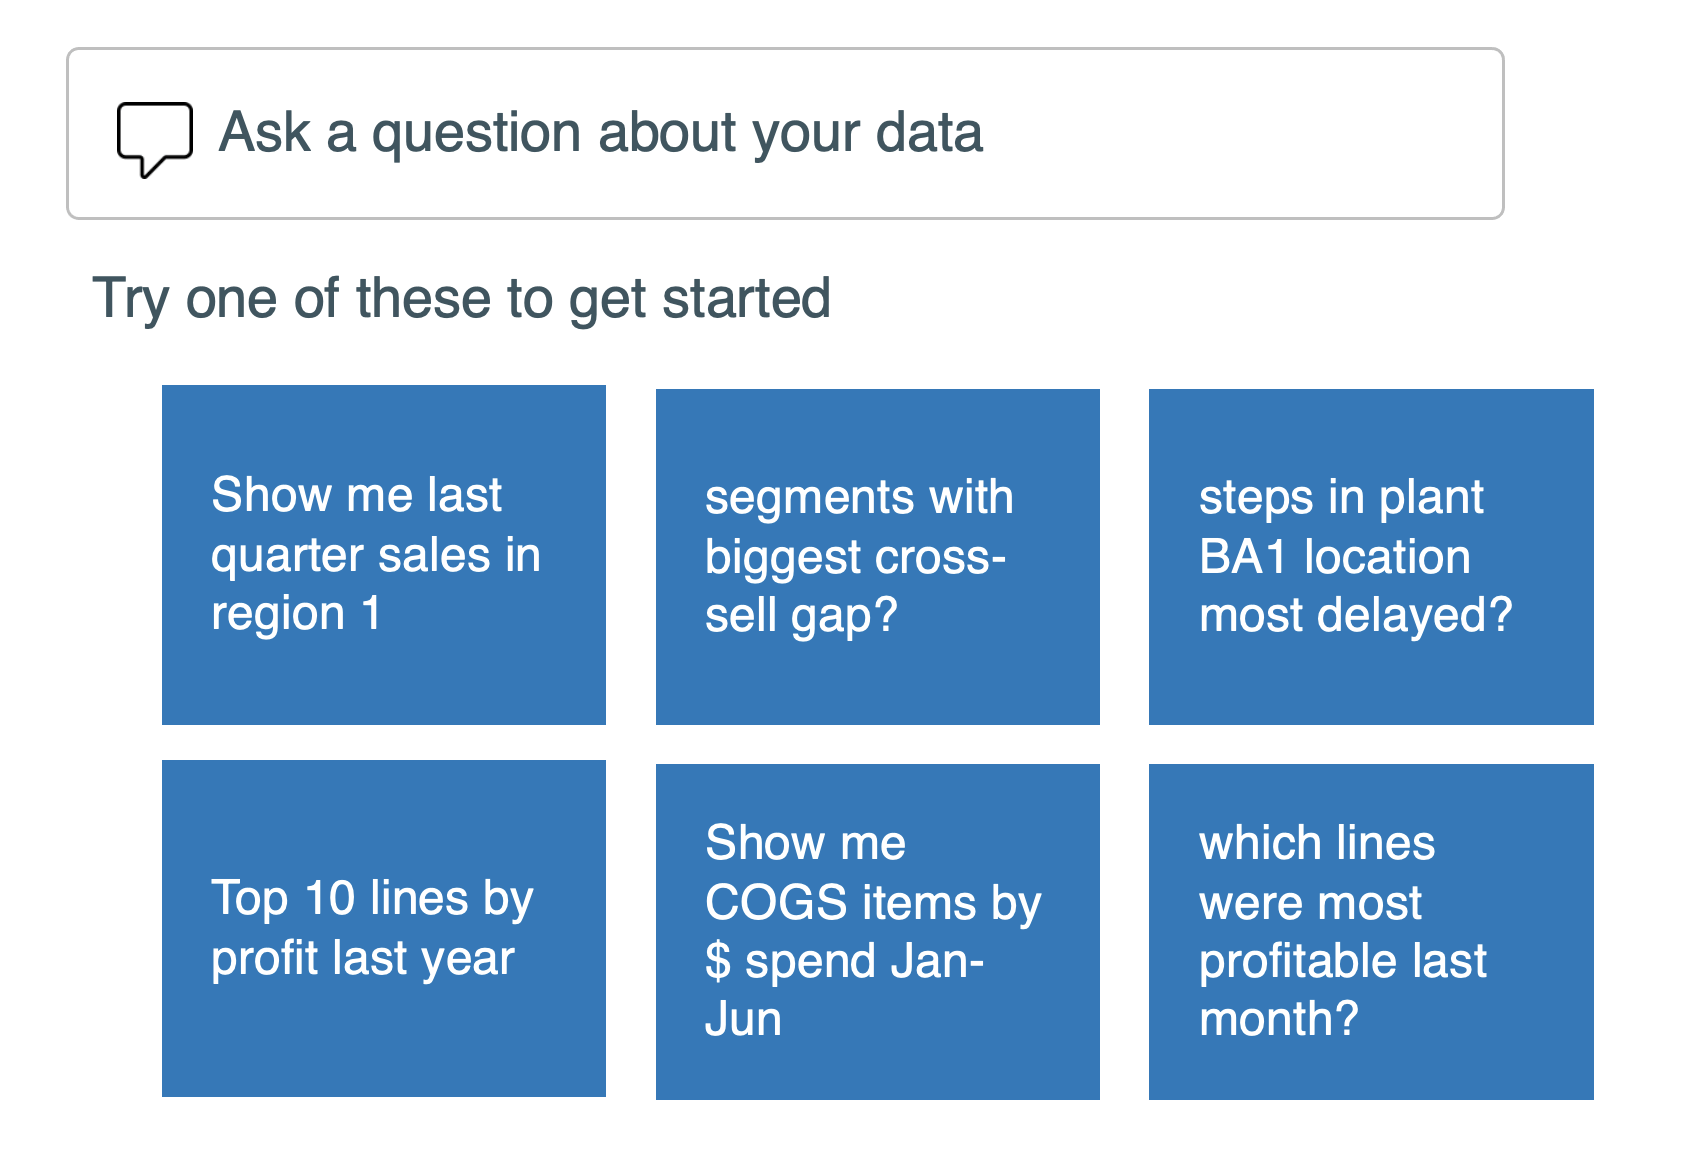
\includegraphics[width=0.6\textwidth]{images/power_bi_Q&A.png}
        \caption{Ejemplo de uso de la función Question Box de \texttt{Power BI}.} \label{fig:power_bi_nlp}
    \end{figure}
%\end{center}

Las razones por las cuales no se hizo uso de Power BI es debido a que en el proyecto no se tienen integrados productos de Microsoft mas que GitHub, lo cual no le quita valor a todo lo que Power BI ofrece, pero se podría hacer un uso más provechoso si en el proyecto se trabajara con un \textit{stack} más enfocado en productos de Microsoft como Azure. Además el costo por una licencia individual para un desarrollador va desde 211 hasta 422 pesos mexicanos, lo cual no es algo que verdaderamente convenga pagar para este tipo de proyecto y las licencias para organizaciones, su precio varias dependiendo de las necesidades. Por último, \textbf{SEDESA} solicitó que todos los módulos del proyecto se encuentren en un mismo sitio, es decir, que se puedan acceder de manera sencilla, por lo que tener únicamente el tablero en una plataforma diferente no es lo más apropiado dado los requerimientos del proyecto.

\subsection{Tableau}
Tableau es una herramienta líder de Business Intelligence (BI) y visualización de datos, diseñada para hacer que el análisis de datos sea accesible e intuitivo para usuarios de distintos niveles. Permite a individuos y organizaciones transformar datos en crudo en tableros de datos interactivos y compartibles, proporcionando información que impulsa la toma de decisiones informadas.\\
A diferencia de las herramientas para creación de tableros de datos, que requieren amplios conocimientos técnicos, Tableau busca dar prioridad a la facilidad de uso, lo que permite a los usuarios técnicos y no técnicos crear visualizaciones y análisis complejos con facilidad, en la Figura \ref{fig:tableua_workload} se muestra como funciona el flujo de trabajo de Tableau. Es compatible con una amplia gama de fuentes de datos, desde hojas de cálculo y bases de datos hasta servicios en la nube, lo que garantiza flexibilidad y conectividad \cite{tableau_help_use_cases} \cite{costello2020prepare}.

\begin{figure}[H]
    \centering
    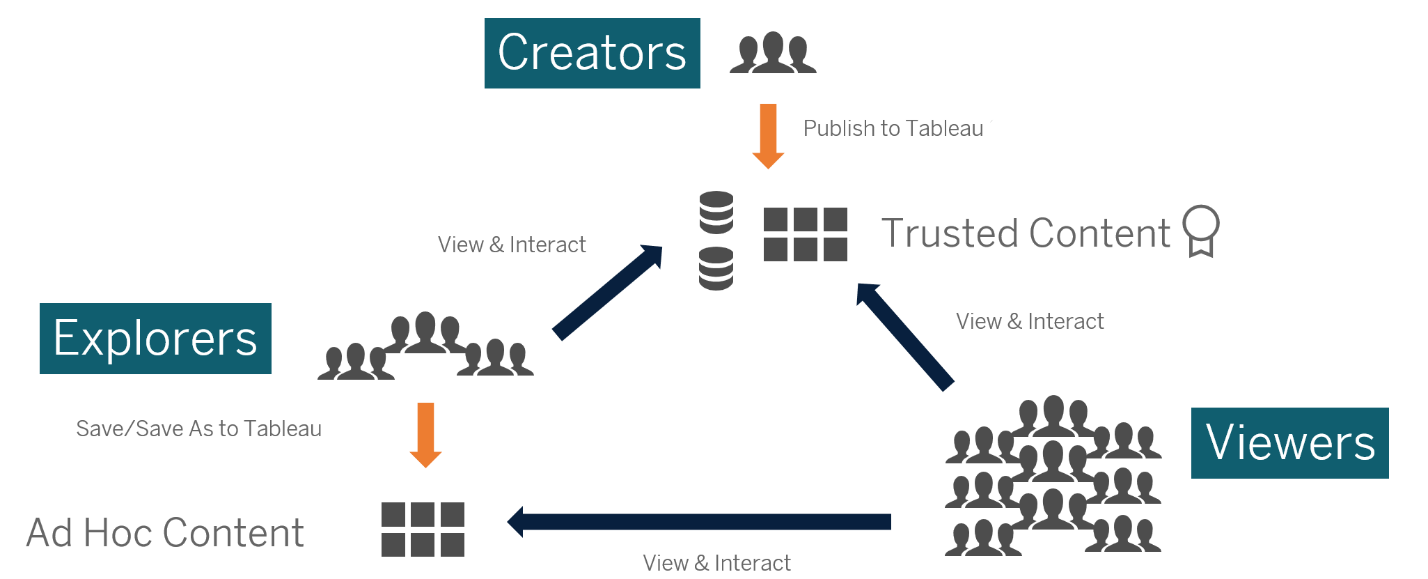
\includegraphics[width=0.7\textwidth]{images/bp_use_cases_1.png}
    \caption{Diagrama del funcionamiento de \texttt{Tableau}.} \label{fig:tableua_workload}
\end{figure}

Entre las características de Tableau, se pueden encontrar las siguientes:
\begin{itemize}
    \item Tableau cuenta con más de 100 conexiones de datos integradas que van desde archivos de texto como Excel a bases de datos como PostgreSQL o herramientas en línea como Google Analytics o Salesforce.com.

    \item Tableau provee una interfaz amigable con el usuario basada únicamente en las acciones de arrastrar y soltar, la interfaz de usuario permite crear fácilmente cuadros, gráficos, mapas y otras visualizaciones sin necesidad de amplios conocimientos previos en programación.

    \item Los usuarios pueden crear visualizaciones dinámicas y atractivas que permiten a los espectadores explorar interactivamente los datos a través de filtros, capacidades de desglose y parámetros personalizables.

    \item Tableau proporciona funciones estadísticas incorporadas, como regresiones lineales, coeficientes de correlación y desviaciones estándar, lo que permite realizar análisis más avanzados dentro de la propia plataforma si es que así se desea.

    \item De manera similar a Power BI, Tableau también ofrece un función que usa procesamiento de lenguaje natural para hacer preguntas sobre los conjuntos de datos que se manipula.

    \item La función que podría ser considera la más útil y atrayente de Tableau, es el poder combinar datos de diferentes fuentes \cite{tableau_help_multiple_connections}. Por ejemplo, combinar datos que se encuentran contenidos en un hoja de calculo de Excel y diferentes datos que se encuentran en PostgreSQL.

    Existen varias formas de combinar datos, cada una con sus propios puntos fuertes y débiles.

    \begin{itemize}
        \item Las relaciones son el método por defecto y pueden utilizarse en la mayoría de los casos, incluso entre tablas con distintos niveles de detalle.

        \item Las uniones combinan tablas añadiendo más columnas de datos a través de estructuras de filas similares. Esto puede provocar la pérdida o duplicación de datos si las tablas tienen diferentes niveles de detalle.

        \item Las mezclas, a diferencia de las relaciones o las uniones, nunca combinan los datos directamente. En su lugar, las mezclas consultan cada fuente de datos de forma independiente, agregan los resultados al nivel adecuado y, a continuación, los presentan juntos visualmente en la vista.
    \end{itemize}

\end{itemize}

Como se puede observar Tableau es un software bastante poderoso que ofrece una amplia gama de herramientas y facilidades para la implementación de tableros datos y distintas visualizaciones.\\
Es una excelente herramienta que se pudo haber utilizado para el desarrollo de este trabajo, pero como se mencionó en el primer capitulo los recursos asignados para la compra de software de pago es limitado y Tableau cuenta con precios de licencias por desarrollador elevados los cuales van desde los 15 hasta los 75 dolares mensuales. De manera similar a lo mencionado anterior anteriormente con Power BI, todos los módulos solicitados por \textbf{SEDESA}, los cuales no se limitan solamente a la visualización de datos, deben estar localizados dentro una misma aplicación o software.

\subsection{Domo Business Intelligence}
Domo es una plataforma analítica en la nube creada para grandes y pequeñas empresas. Está adecuadamente equipada para cualquier tipo de institución debido a su amplio conjunto de funciones que cubren todos los requisitos que un software de visualización de datos debe cubrir; de seguridad, gobernanza, tableros de datos y generación de reportes, todo ello en un entorno colaborativo. Domo tiene un paquete de gestión empresarial que se integra con múltiples fuentes de datos que ayudan a las instituciones a tomar decisiones cruciales a través de los servicios que Domo tiene para ofrecer \cite{robb2022domo}.\\

Domo posee funciones similares a las ya mencionadas en Tableau y Power BI, pero además de estas, las principales funciones que lo diferencian de sus competidores son las siguientes \cite{graphable_domo_analytics}:

\begin{itemize}
    \item \textbf{Transformación de datos (Ingeniería de datos)}\\
    Domo contiene funciones enfocadas en la Ingeniería de datos para hacer operaciones con los datos manipulados como Magic ETL \footnote{ETL es el acronimo correspondiente al término \textit{Extract, Transform and Load}} (flujos ETL de arrastrar y soltar), SQL dataflows (flujos de datos creados a partir de scripts de SQL) y vistas interactivas de conjuntos de datos están siempre disponibles, todo estos flujos de datos pueden ser creados a partir de varias fuentes de datos desde Google Sheets, MySQL y servicios en la nube como Amazon Web Services. También cuenta con estudio de ciencia de datos, aprendizaje automático automatizado, catálogo de instancias visual/en tiempo real e interactivo, lo cual permiten a los usuarios realizar de tableros y/o visualizaciones de datos de manera más rápida y eficaz.

    
    \item \textbf{Elaboración de Informes y Tableros de Datos}\\
    Domo ofrece una extensa variedad de recursos para la visualización de datos, que incluyen más de 150 tipos de gráficos, más de 7,000 opciones de mapas personalizables, capacidades de análisis mediante la función de arrastrar y soltar, así como la creación de contenido con cálculos personalizados. Estos elementos pueden ser compartidos de manera simple, y la implementación de tableros de datos se realiza de manera sencilla.

    \item \textbf{Creación de aplicaciones interactivas}\\
    Domo provee un servicio para crear aplicaciones interactivas las cuales pueden ser modificadas a partir de la producción de código y/o sin la necesidad de la programación en ReactJS, estas permiten a los usuarios ir más allá del conjunto de visualizaciones y tableros de datos estándar para capturar visualmente incluso los procesos empresariales más específicos y complejos, aprovechando al mismo tiempo todas las capacidades de Domo, incluidas la gobernanza y la seguridad.

    \item  \textbf{Compatibilidad con dispositivos moviles}\\
    Domo también está disponible para dispositivos moviles tanto en iOS como en Android. Tal vez, implementar y desarrollar proyectos en este tipo de dispositivos no es lo más conveniente y eficaz, pero la portabilidad que estos conceden al momento de presentar tableros y/o visualizaciones es poderoso. 
    
    
\end{itemize}

Existen ejemplos en linea dónde se puede observar la capacidad de uso de Domo, desde simples tableros de una sola página no interactivos, hasta aplicaciones interactivas de varias páginas:

\begin{itemize}
    \item En la página \url{https://www.domo.com/dashboard/marketing} ofrece un ejemplo de de como se podría implementar un tablero de datos especializado en marketing que brinda a los usuarios una herramienta para la integración, transformación, análisis y visualización de datos de manera eficiente y efectiva. Este tablero está diseñado específicamente para mostrar como un Domo puede usarse para implementar un tablero de datos que puedan cubrir las necesidades de los profesionales del marketing al proporcionar una visión completa y en tiempo real del rendimiento de sus campañas y estrategias, esto gracias al uso de diversas gráficas que van desde tablas, hasta mapas geográficos, todos ellos personalizados de manera avanzada.
\end{itemize}

Como se puede observar Domo es una gran herramienta que proporciona una diversa cantidad de funciones para la implementación de tableros de datos, siendo más permisiva que Tableau y Power BI en cuestión de personalización.\\
Una de las desventajas es su curva de aprendizaje, poder implementar un tablero de datos funcional y visualmente atractivo lleva tiempo considerable debido a que en algunos casos se requiere de la programación adicional en ReactJS.\\
Además de que Domo tiene un costo mensual más elevado (300 dolares al mes) al que manejan Tableau y Power BI, y el soporte y documentación que se puede encontrar es más limitado.\\

Por estas razones se decidió no hacerse de su uso, ya que lo más acertado era que se requeriría de programar, se optó por adquirir una biblioteca de pago como AmCharts, la cual sólo requiere de un pago único.

\section{Resumen}
En este capítulo, se realizó una exhaustiva revisión de las tecnologias usados hoy en día para la implementación de tableros de datos, revisando herramientas tanto de código abierto como de pago. \\
Se describió una visión general de las características clave que se buscan en un software para el desarrollo de tableros, incluyendo plantillas predeterminadas, seguridad de datos, procesamiento en tiempo real, personalización e integración, una variedad extensa gráficos, opciones para compartir y capacidad de exportación.
\\

La exploración de herramientas de Software Open Source se centró en tres soluciones prominentes: Tableau Public, Google Data Studio y Grafana. Cada herramienta fue analizada en términos de características, ventajas y desventajas. A pesar de sus beneficios, se identificaron limitaciones específicas como la falta de privacidad de datos y personalización de los tableros, que hicieron que estas opciones no fueran las más adecuadas para la implementación del proyecto en cuestión.\\

La revisión de Software de Paga se centró en tres principales herramientas: Microsoft Power BI, Tableau y Domo. Se destacaron características clave, como la capacidad de integración, la facilidad de uso, las funciones avanzadas de procesamiento de datos y las opciones de personalización. Sin embargo, debido a consideraciones como la falta de integración con otros productos y el costo asociado, se tomó la decisión de explorar otras opciones para la implementación del tablero de datos\\

En última instancia, este capítulo proporcionó una base sólida para la toma de decisiones al analizar en detalle las opciones disponibles en el mercado y considerar cuidadosamente las necesidades y restricciones específicas del trabajo hecho. 